This feature has been contributed to \NAMD\ by the following authors:

\begin{quote}
   Surjit B. Dixit and Christophe Chipot          \\[0.4cm]
   {\it Equipe de dynamique des assemblages membranaires }\\
   {\it Institut nanc\'eien de chimie mol\'eculaire,  }\\
   {\it UMR CNRS/UHP 7565,                            }\\
   {\it Universit\'e Henri Poincar\'e,                }\\
   {\it BP 239,                                       }\\
   {\it 54506 Vand\oe uvre--l\`es--Nancy cedex, France}
\end{quote}



\subsubsection{Introduction and theoretical background}


A method to perform alchemical free energy perturbation (\FEP)
~\cite{zwan_54_1,Beveridge.89,Gunsteren.89,Straatsma.92,Kollman.93,Gilson.97,
Mark.98,chip_01_1} within \NAMD\ has now been implemented. 
In \FEP, the free energy difference between two states,
$a$ and $b$, is expressed by:

\begin{equation}
\label{master}
\Delta A_{a \rightarrow b} = -k_B T \ \ln
\left< \exp\left[-\frac{{\cal H}_b({\bf r}, {\bf p}) - 
                         {\cal H}_a({\bf r}, {\bf p})}
                        {k_B T}\right]
\right>_a
\end{equation}

wherein $k_B$ is the Boltzmann constant, $T$ is the temperature,
and ${\cal H}_a({\bf r}, {\bf p})$ and ${\cal H}_b({\bf r}, {\bf p})$
are the Hamiltonians characteristic of states $a$ and $b$, respectively.
$\left< \cdots \right>_a$ denotes an ensemble average over configurations
representative of the initial state, $a$.
In practice, the transformation between the two thermodynamic states
is replaced by a series of transformations between non--physical,
intermediate states along a pathway that connects $a$ to $b$.
This pathway is characterized by a variable, referred to as
``coupling parameter'',~\cite{Beveridge.89,Mark.98,king_93_1} 
$\lambda$, that makes the free energy
a continuous function of this parameter between $a$ and $b$:

\begin{equation}
\Delta A_{a \rightarrow b} = -k_B T \ \sum_{k = 1}^N \ln
\left< \exp\left[-\frac{{\mathcal H}({\bf r}, {\bf p}; \lambda_{k+1}) - 
                        {\mathcal H}({\bf r}, {\bf p}; \lambda_k)}
                        {k_B T}\right]
\right>_k
\end{equation}

Here, $N$ stands for the number of intermediate states, or ``windows''
between the initial and the final states.


In a typical \FEP\ setup, that involves the transformation
of one chemical species 
into another one, the atoms in the molecular topology can be 
separated into three groups: (i) a group of atoms that do not change 
during the simulation --- \eg the environment, (ii) 
those atoms describing the initial state, $a$, of the system, and (iii) 
those that correspond to the final state, $b$, at the end of the 
alchemical transformation. 
The atoms representative of state $a$
do not interact with those of state $b$ throughout the 
entire molecular dynamics simulation. 
Such a setup, in which atoms pertaining to both the initial and the
final states of the system are present in the molecular topology file --- \ie 
the {\tt psf} file --- is referred to as ``dual topology'' 
paradigm.~\cite{Axelsen.98,Pearlman.94}
The hybrid Hamiltonian of the system, which is a function of the
coupling parameter $\lambda$, that smoothly connects state $a$
to state $b$, is evaluated as:

\begin{equation}
{\mathcal H}(\lambda) = {\mathcal H}_0 
                      + \lambda {\mathcal H}_a 
                      + (1-\lambda) {\mathcal H}_b
\end{equation}

where ${\mathcal H}_a$ is the Hamiltonian for the group of atoms representative
of the initial state, $a$, and ${\mathcal H}_b$ characterizes the final state,
$b$. ${\mathcal H}_0$ is the Hamiltonian for those atoms that do not undergo any 
transformation during the MD simulation.


For instance, in a transformation involving the mutation of an
alanine side chain into that of glycine, using the \FEP \ methodology, 
the topology of both the methyl group of alanine
and the hydrogen borne by the C$_\alpha$ in glycine co--exist
throughout the simulation (see Figure~\ref{fig:dual_top}).


\begin{figure}[ht]
  \center{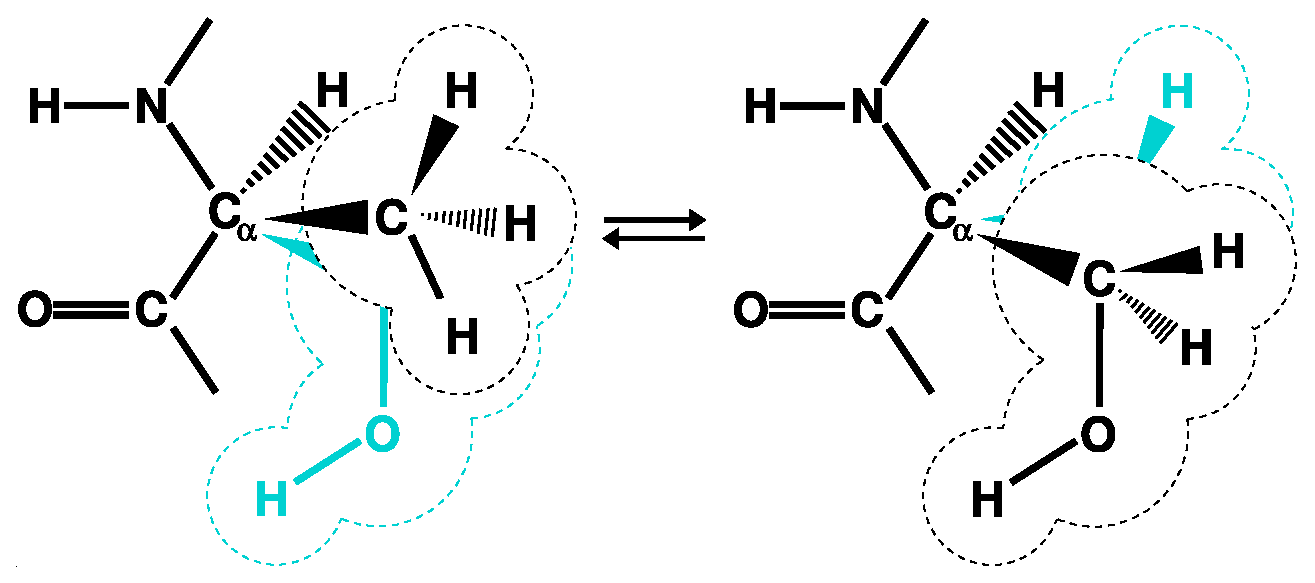
\includegraphics[width=14.5cm]{figures/dual_top}}
  \caption{Dual topology description for an alchemical simulation.
         Case example of the mutation of alanine into glycine.
         The lighter color denotes the non--interacting, alternate
         state.}
  \label{fig:dual_top}
\end{figure}


The energy and forces
are defined as a function of $\lambda$, in such a fashion that 
the interaction of the methyl group of alanine with the rest of 
the protein is effective at the beginning of the simulation,
\ie $\lambda$ = 0, while
the glycine C$_\alpha$ hydrogen does not interact with the rest
of the protein, and {\it vice versa} at the end of the
simulation, \ie $\lambda$ = 1.
For intermediate values of $\lambda$, both the alanine and the glycine
side chains participate in the non--bonded interactions with the rest 
of the protein, scaled on the basis of the current value of $\lambda$.
It should be emphasized that these side chains, however,
do not interact with each other.


It is, therefore, necessary to exclude {\it explicitly} in the setup
those atoms 
that are created from those that will be annihilated in the 
course of the \FEP\ calculation (see ``A tutorial to set up 
alchemical free energy perturbation calculations in \NAMD''
available from the \NAMD\ website).


It is also worth noting that
the free energy calculation does not alter intramolecular
potentials, \ie bond stretch, valence angle deformation, torsions
{\it etc}, during the simulation.
In calculations targetted at the estimation
of free energy differences between two states characterized by
distinct environments --- \eg a ligand bound to a protein in
the first simulation,
and solvated in water, in the second --- as is the 
case for most free energy calculations that make use of a thermodynamic 
cycle, perturbation of intramolecular terms, 
\eg chemical bonds, can be safely
avoided.~\cite{Boresch.99a}



\subsubsection{Implementation of free energy perturbation in \NAMD}


The procedure implemented in \NAMD\ is particularly
adapted for performing free 
energy calculations that split the reaction path into a number of non--physical,
intermediate $\lambda$--states, or ``windows''. Separate simulations 
can be started for each window.
Alternatively, the {\sc Tcl} scripting ability of 
\NAMD\ can be employed advantageously
to perform the complete simulation in a single run.
An example making use of such script is supplied at the end 
of this section.


The following keywords can be used to control free 
energy calculations aimed at alchemical transformations. 

\begin{itemize}

\item
\NAMDCONFWDEF{fep}{ Is alchemical \FEP\ to be performed? }
{{\tt on} or {\tt off}}
{{\tt off}}
{Turns on Hamiltonian scaling and ensemble averaging for alchemical \FEP.}

\item
\NAMDCONF{lambda}{ Coupling parameter value }
{positive decimal between 0.0 and 1.0}
{The coupling parameter value determining the progress of the
perturbation. The non--bonded interactions involving the atoms vanishing
in the course of the MD simulation are scaled by (1-{\tt lambda}), while
those of the growing atoms are scaled by {\tt lambda}.}

\item
\NAMDCONF{lambda2}{Coupling parameter comparison value}
{positive decimal between 0.0 and 1.0}
{The {\tt lambda2} value corresponds to the coupling parameter to be
used for sampling in the next window.  The free energy difference
between {\tt lambda2} and {\tt lambda} is calculated.  Through simulations
at progressive values of {\tt lambda} and {\tt lambda2} the total free
energy difference may be determined.}

\item
\NAMDCONFWDEF{fepEquilSteps}{Number of equilibration steps in the window, 
before data collection}
{positive integer less than {\tt numSteps} or {\tt run}}
{0}
{In each window {\tt fepEquilSteps} steps of equilibration can be
performed before ensemble averaging is initiated. The output also contains
the data gathered during equilibration and is meant for analysis of
convergence properties of the \FEP\ calculation.}

\item
\NAMDCONFWDEF{fepFile}{{\tt pdb} file with perturbation flags}
{filename}
{coordinates}
{{\tt pdb} file to be used for indicating the \FEP\ status for each of
the atoms pertaining to the system. 
If this parameter is not declared specifically, then the
{\tt pdb} file containing the initial coordinates specified by
{\tt coordinates} is utilized for this information.}

\item
\NAMDCONFWDEF{fepCol}{Column in the {\tt fepFile} that carries 
                      the perturbation flag}
{X, Y, Z, O or B}
{B}
{Column of the {\tt pdb} file to use for retrieving the \FEP\ status 
of each atom, \ie a flag that indicates which atom will be perturbed
in the course of the simulation.
A value of {\tt -1} in the specified column indicates the atom will
vanish during the \FEP\ calculation, whereas a value of {\tt 1} 
indicates that the atom will grow.}

\item
\NAMDCONFWDEF{fepOutFreq}{Frequency of \FEP\ energy output in time--steps}
{positive integer}
{5}
{Every {\tt fepOutFreq} number of MD steps, the output file
{\tt fepOutFile} is updated by dumping energies that are
used for ensemble averaging.
This variable could be set to {\tt 1} to include all the 
configurations for ensemble averaging. Yet, it is recommended
to update {\tt fepOutFile}  energies at longer intervals
to avoid large correlation between consecutive configurations.}

\item
\NAMDCONFWDEF{fepOutFile}{\FEP\ energy output filename}
{filename}
{outfilename}
{An output file named {\tt fepOutFile}.fep, generated by \NAMD,
contains the \FEP\ energies, dumped every {\tt fepOutFreq} steps.}

\end{itemize}


\noindent
{\it Note}: Free energy calculations that rely upon equation~({\ref{master}})
make use of an average temperature, which, in principle, should coincide with
the value of the thermostat. Rather than employing the computed average of $T$,
$\Delta A_{a \rightarrow b}$ is estimated with the target value of the
temperature defined by the user. It is, therefore, necessary to activate
some constant--temperature scheme to carry out \FEP\ calculations. 



\subsubsection{Example of an input file for running \FEP\ alchemical transformations}


The following example illustrates the use of {\sc Tcl} scripting for running
the alchemical \FEP\ feature of \NAMD: 

\begin{verbatim}
fep		on  
fepfile		ion.fep
fepCol		X
fepOutfile	ion.fepout
fepOutFreq	5
fepEquilSteps	5000

set step 0.0
set dstep 0.1

while {$step <= 0.9} {
 lambda $step
 set step [expr $step+$dstep]
 lambda2 $step
 run  10000
}
\end{verbatim}

\noindent
Here, the {\tt pdb} file read by \NAMD\ to extract the information
about perturbed atoms is {\tt biotin.fep}. The pertinent information 
is present in the {\tt X} column. The output file of the free energy
calculation is {\tt biotinr.fepout}, in which energies are written
every {\tt 5} steps.
$\delta \lambda$, the width of the windows, is set to {\tt 0.1}.
{\tt 5000} MD steps are performed in each window to
equilibrate the system. In this particular instance, 
the current value of $\lambda$
is controlled by the statement {\tt set step}. 
The \FEP\ calculation is run until $\lambda$ reaches the
value {\tt 0.9}. In every window, {\tt 10000} MD steps
are performed.


\subsubsection{Description of \FEP\ simulation output }

The {\tt fepOutFile} contains electrostatic and van der Waals energy
data calculated at $\lambda$ and $\lambda2$, written every
{\tt fepOutFreq} steps. The column {\tt dE} is the instantaneous energy
difference for the current configuration. {\tt dE\_avg} and {\tt dG}
are the accumulated energy ensemble average and the corresponding
free energy at the current time step, respectively.
The temperature is specified in the penultimate column. Upon completion
of {\tt fepEquilSteps} steps, the calculation of {\tt dE\_avg} and 
{\tt dG} is restarted. The accumulated net free energy change is output
at each $\lambda$--value and at the end of the simulation. The cumulative
average energy {\tt dE\_avg} value may be summed using, for instance, the 
trapezoidal rule, or a Gaussian quadrature, to obtain an approximate 
TI estimate for the free energy change during the run.


